\chapter{Estratégias de RVD/B}
\label{sec:estrategias_rvdb}

Este capítulo apresenta as estratégias adotadas para a condução da missão de \gls{rvdb}, aproximação e acoplamento entre a espaçonave perseguidora e o alvo em órbita circular.
As estratégias de \gls{rvdb} são decompostas em quatro eixos principais:
\begin{enumerate}[label=(\roman*)]
  \item \textbf{Estratégia orbital}: define como o  reduz a diferença de ângulo entre as espaçonaves e realiza a aproximação longa através da transferência orbital;
  \item \textbf{Estratégia de aproximação relativa}: responsável pela transição entre aproximação longa, aproximação curta e aproximação final;
  \item \textbf{Estratégia de controle de atitude}: responsável por manter o alinhamento de atitude do perseguidor em relação ao alvo;
  \item \textbf{Estratégia de operação do manipulador robótico}: determina o uso do \gls{mr} na fase final, que ocorre a captura e acoplamento.
\end{enumerate}

\section{Estratégia orbital}
\label{sec:estrategia_orbital}

A missão considerada neste trabalho segue o encadeamento clássico das operações de \gls{rvdb} entre uma espaçonave perseguidora e um alvo em órbita circular \cite{fehse2003}.
Nesta etapas ocorrem:

\begin{enumerate}[label=(\roman*)]
  \item lançamento e injeção do perseguidor em órbita circular terrestre baixa;
  \item redução do ângulo de fase entre as espaçonaves;
  \item transferência de órbita.
\end{enumerate}

\subsection{Premissas orbitais}

Nessa etapa, é realizada a aproximação longa e toda a movimentação do perseguidor é realizada no referencial inercial, utilizando o problema de dois corpos.
Considera-se que o perseguidor foi injetado pelo veículo lançador em sua órbita de injeção, a qual é circular e coplanar em relação à orbita do alvo.

\begin{figure}[H]
\centering

\includegraphics[width=1\linewidth]{2 Estrategia de RVDB/Imagens/1 Posicao espaconaves injecao orbital.png}
\caption{Posição inicial das espaçonaves.}
\label{fig:injecao_orbita_inicial}
\end{figure}

Na Figura~\ref{fig:injecao_orbita_inicial} é possível observar a diferença de ângulo entre as espaçonaves durante a injeção do perseguidor em sua órbita inicial.
A diferença de ângulo entre as espaçonaves no início da operação é reduzida através da diferença da velocidade entre as espaçonaves (\emph{drift} orbital).
Ao obter uma diferença de ângulo adequada o suficiente, realiza-se duas manobras impulsivas que conduzem o perseguidor a uma nova órbita, de raio orbital inferior ao do alvo.
Além disso, o perseguidor estará atrasado em relação ao alvo.

\begin{figure}[H]
\centering
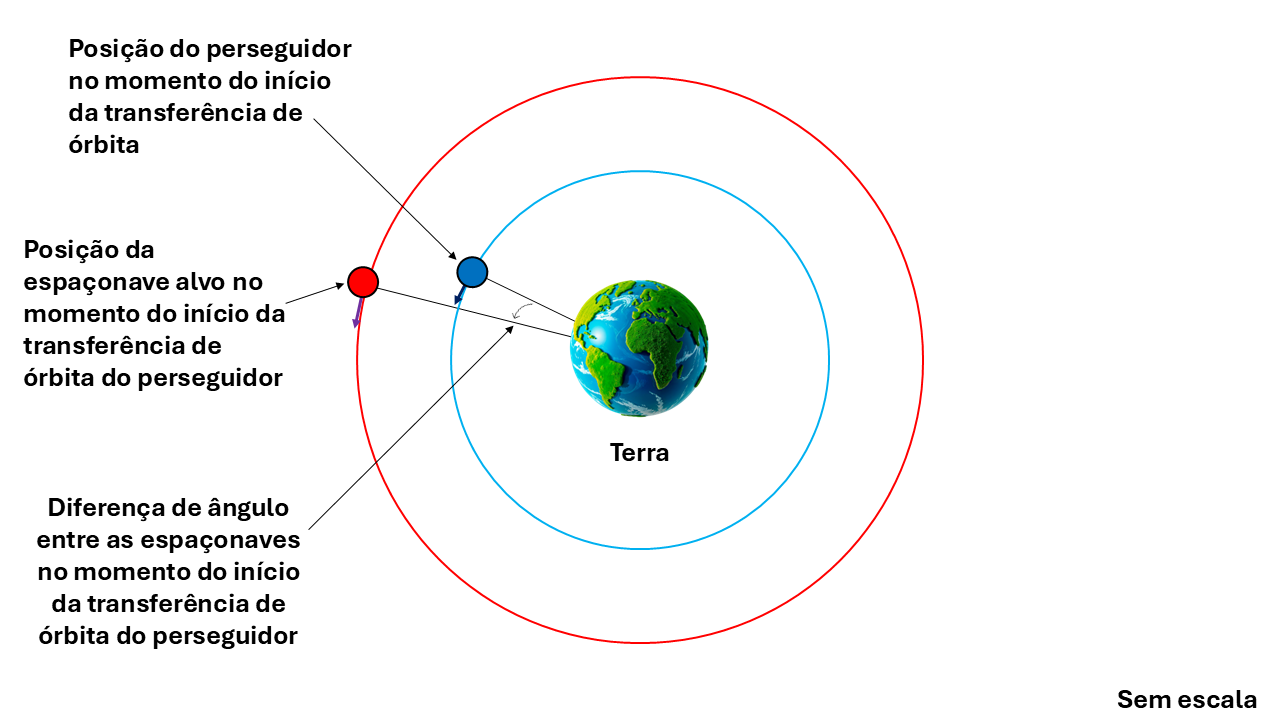
\includegraphics[width=1\linewidth]{2 Estrategia de RVDB/Imagens/2 Injecao orbita antes da transf de orbita.png}
\caption{Momento do início da transferência orbital.}
\label{fig:transf_orbita}
\end{figure}

Por sua vez, a Figura~\ref{fig:transf_orbita} demonstra a redução da diferença de fase entre as espaçonaves.

\subsection{Parâmetros orbitais absolutos}

A Tabela~\ref{tab:parametros_orbitais_iniciais} contempla todos os parâmetros orbitais durante essa primeira fase de operação das espaçonaves.


\begin{longtable}{lrr}
\caption{Constantes gravitacionais, altitudes, raios orbitais e elementos orbitais iniciais.}
\label{tab:parametros_orbitais_iniciais}\\
\hline
\textbf{Variável} & \textbf{Valor} & \textbf{Unidade} \\
\hline
\endfirsthead

\caption*{(Continuação) Constantes gravitacionais, altitudes, raios orbitais e elementos orbitais iniciais.}\\
\hline
\textbf{Variável} & \textbf{Valor} & \textbf{Unidade} \\
\hline
\endhead

\hline
\endfoot

\hline
\endlastfoot

\multicolumn{3}{l}{\textbf{Constantes e parâmetros planetários}} \\
\hline
$\mu_{\text{Terra}}$                               & $3.986004418\times 10^{14}$ & m$^{3}$/s$^{2}$ \\
$R_{\text{Terra}}$                                & $6378.14$                   & km \\
\hline
\multicolumn{3}{l}{\textbf{Altitudes e raios orbitais}} \\
\hline
Altitude inicial do perseguidor                   & $500.00$                    & km \\
Altitude do perseguidor após transferência orbital & $559.90$                   & km \\
Altitude inicial do alvo                          & $600.00$                    & km \\
Raio orbital inicial do perseguidor               & $6878.14$                   & km \\
Raio orbital do perseguidor após transferência orbital & $6938.04$              & km \\
Raio orbital inicial do alvo                      & $6978.14$                   & km \\
\hline
\multicolumn{3}{l}{\textbf{Longitudes inerciais iniciais}} \\
\hline
Longitude inercial inicial do perseguidor         & $-7.00 / -0.12$             & deg / rad \\
Longitude inercial inicial do alvo                & $0.00 / 0.00$               & deg / rad \\
\hline
\multicolumn{3}{l}{\textbf{Elementos orbitais iniciais do alvo}} \\
\hline
Semi-eixo maior $a_{\text{alvo}}$                 & $6978.14$                   & km \\
Excentricidade $e_{\text{alvo}}$                  & $0.00$                      & -- \\
Inclinação $i_{\text{alvo}}$                      & $0.00 / 0.00$               & deg / rad \\
Longitude do nó ascendente $\Omega_{\text{alvo}}$ & $0.00 / 0.00$               & deg / rad \\
Argumento do perigeu $\omega_{\text{alvo}}$       & $0.00 / 0.00$               & deg / rad \\
Anomalia verdadeira inicial $\nu_{\text{alvo},0}$ & $0.00 / 0.00$               & deg / rad \\
\hline
\multicolumn{3}{l}{\textbf{Elementos orbitais iniciais do perseguidor}} \\
\hline
Excentricidade $e_{\text{perseguidor}}$ & $0.0$ & -- \\
Inclinação $i_{\text{perseguidor}}$& $0.00 / 0.00$               & deg / rad \\
Longitude do nó ascendente $\Omega_{\text{perseguidor}}$ & $0.00 / 0.00$ & deg / rad \\
Argumento do perigeu $\omega_{\text{perseguidor}}$ & $0.00 / 0.00$& deg / rad \\
Anomalia verdadeira inicial $\nu_{\text{perseguidor},0}$ & $-7.00 / -0.12$& deg / rad \\

\end{longtable}

\section{Estratégia de aproximação relativa}
\label{sec:estrategia_orbital_global}

Ao final da manobra de transferência orbital, o perseguidor é inserido em uma nova órbita e permanece em regime de \textit{drift} por um intervalo de tempo predeterminado.
Nesse intervalo, a dinâmica é propagada essencialmente pelo problema de dois corpos, enquanto são realizadas checagens de posição e velocidade relativa em relação ao alvo.

\subsection{Aproximação curta}
\label{sec:aproximacao_curta}

Somente após essa fase de \textit{drift} é que se considera o início da aproximação curta.
O estado do perseguidor ao término do \textit{drift} é tomado como condição inicial no referencial \gls{lvlh} do alvo, e a dinâmica relativa passa a ser descrita pelo modelo linearizado \gls{hcw}.
A partir desse instante, a lei de controle \gls{pd} assume realizando correções nas componentes radial, ao longo da órbita e transversal.

\subsection{Aproximação final}
\label{sec:aproximacao_final}

A aproximação final corresponde ao trecho final da manobra translacional, já no interior da região de captura em \gls{lvlh} centrado no alvo.
Nessa fase, o perseguidor encontra-se a poucos metros da porta de acoplamento e as condições de posição, velocidade relativa e atitude são mais restritivas do que nas etapas anteriores.
O objetivo principal é reduzir os erros residuais de posição e velocidade até atingir um estado quase estacionário em relação ao alvo para que ocorra a atuação do manipulador robótico.

Assim que o perseguidor insere o efetuador final na porta de acoplamento, a aproximação final é finalizada, assim como toda a missão.
A Tabela~\ref{tab:parametros_pos_TH} demonstra os valores obtidos durante a aproximação curta e final.

\begin{table}[H]
\centering
\renewcommand{\arraystretch}{1.2}
\caption{Parâmetros relativos alvo--perseguidor durante a aproximação curta.}
\label{tab:parametros_pos_TH}
\begin{tabular}{lrr}
\hline
\textbf{Variável} & \textbf{Valor} & \textbf{Unidade} \\
\hline
\multicolumn{3}{l}{\textbf{Condições relativas após TH}} \\
\hline
$\Delta r_{\text{radial,TH}}$& $-100.00$& m \\
$\Delta r_{\text{along,TH}}$& $-500.00$& m \\
$\Delta r_{\text{cross,TH}}$& $0.00$& m \\
\hline
\multicolumn{3}{l}{\textbf{Limites de velocidade relativa}} \\
\hline
$v_{\text{rel,max}}(d \leq 1000\,\text{m})$ & $0.30$ & m/s \\
$v_{\text{rel,max}}(d \leq 50\,\text{m})$& $0.03$ & m/s \\
\hline
\multicolumn{3}{l}{\textbf{Condições de atitude inicial}} \\
\hline
$q_{\text{alvo},0}$& $[1,\;0,\;0,\;0]$ & -- \\
$\boldsymbol{\phi}_{\text{chr},0}$ (Euler) & $[7,\;8,\;9]$     & deg \\
$q_{\text{chr,des}}$& $[1,\;0,\;0,\;0]$ & -- \\
\hline
\end{tabular}
\end{table}

A Tabela~\ref{tab:aproximacao_final} explicita os valores obtidos durante a aproximação final.
\begin{table}[H]
\centering
\renewcommand{\arraystretch}{1.2}
\caption{Condições de referência na aproximação final em LVLH.}
\label{tab:aproximacao_final}
\begin{tabular}{lrr}
\hline
\textbf{Variável} & \textbf{Valor} & \textbf{Unidade} \\
\hline
\multicolumn{3}{l}{\textbf{Posição em LVLH (alvo como referência)}} \\
\hline
Posição do alvo em LVLH, $\vec r_{\text{alvo}}$ &
$[0.00,\;0.00,\;0.00]$ & m \\
Posição do COM da base em LVLH, $\vec r_{\text{base}}$ &
$[0.00,\;0.00,\;0.70]$ & m \\
\hline
\multicolumn{3}{l}{\textbf{Velocidade relativa na aproximação final}} \\
\hline
Velocidade relativa base–alvo, $\dot{\vec r}_{\text{rel}}$ &
$[0.00,\;0.00,\;0.00]$ & m/s \\
\hline
\end{tabular}
\end{table}

\section{Estratégia de controle de atitude}
\label{sec:controle_atitude}

A estratégia de controle adotada combina o controle \gls{pd} aplicado à dinâmica relativa em \gls{lvlh} com controle \gls{pd} de atitude da base, operando em dois modos distintos: com o \gls{mr} travado (dinâmica de corpo rígido) e com o \gls{mr} em operação (dinâmica acoplada base--MR).
Na fase final, um controle \gls{pd} adicional atua nas juntas do manipulador para executar a manobra de captura.

\subsection{Controle PD na dinâmica relativa}
\label{sec:controle_PD_HCW}

A aproximação relativa em \gls{lvlh} é descrita, nas vizinhanças da órbita de fase, por um modelo linearizado do tipo \gls{hcw}, que relaciona posição e velocidade relativas do perseguidor em relação ao alvo.
Sobre esse modelo é definida uma lei de controle PD em translação, que atua sobre o vetor de erro de posição relativa e sobre a velocidade relativa.

O objetivo é conduzir o perseguidor de um estado inicial de \textit{drift} até a região de captura, respeitando os limites de velocidade relativos estabelecidos.
As saídas desse controlador são comandos de translação (equivalentes a impulsos) que definem a trajetória relativa desejada para a base.

\subsection{Controle de atitude com MR travado}
\label{sec:controle_atitude_Euler}

Quando o \gls{mr} permanece travado em configuração fixa, o conjunto base--\gls{mr} é tratado como um corpo rígido.
Nessa condição, a atitude da base é controlada pela dinâmica de Euler e o controle de atitude atua diretamente sobre os torques da base física, sem contribuição de reações articulares.
A estratégia consiste em aplicar uma lei de controle PD de atitude, formulada em termos de um quaternion de erro entre a orientação da base e uma orientação de referência associada ao alvo, e da velocidade angular medida no sistema corpo.
Esse controle é responsável por manter a base alinhada com o alvo durante a aproximação curta, enquanto o controle translacional em \gls{lvlh} define a trajetória relativa.

\subsection{Controle de atitude com dinâmica acoplada}
\label{sec:controle_atitude_Lagrange}

No modo operacional, o \gls{mr} passa a se movimentar para executar a manobra de captura.
A dinâmica do sistema deixa de ser equivalente à de um corpo rígido e passa a ser descrita pela formulação de Lagrange com coordenadas generalizadas que incluem a atitude da base e as juntas do manipulador.
Os movimentos articulares geram torques internos que aparecem como reações na base, alterando a sua atitude.

A estratégia de controle mantém a mesma lei PD de atitude aplicada às coordenadas da base, dessa forma, o mesmo controlador que estabiliza a atitude quando o \gls{mr} está travado passa a atuar também como compensador das reações provenientes dos movimentos das juntas.
Assim, o controle de atitude deve ao mesmo tempo seguir a referência de apontamento em relação ao alvo e rejeitar as perturbações internas induzidas pela operação do manipulador.

\subsection{Controle das juntas do manipulador na aproximação final}
\label{sec:controle_juntas_MR}

Na fase de aproximação final, após o perseguidor estar inserido na região de captura com atitude estabilizada, um controlador adicional atua nas juntas do manipulador para rastrear trajetórias articulares de referência associadas às fases de posicionamento, alinhamento fino e inserção.
Esse controlador é do tipo PD no espaço de juntas, definido a partir do erro entre os ângulos articulares medidos e os ângulos desejados, bem como das velocidades articulares.

O objetivo é garantir que o efetuador siga trajetórias suaves, evitando saturações de torque e limitando as reações transmitidas à base.
Dessa forma, o controle das juntas complementa o controle de atitude da base: enquanto a base procura manter o apontamento desejado e compensar as reações globais, o controlador em espaço de juntas realiza a manobra local necessária para alinhar a ferramenta com a porta e completar a captura.

\section{Estratégia de operação do manipulador robótico}
\label{sec:estrategia_operacao_MR}

A operação do \gls{mr} é organizada de forma coerente com as fases de aproximação relativa em \gls{lvlh} e com os critérios de atitude da espaçonave.
Em termos operacionais, o manipulador permanece inicialmente travado (modo não-operacional), de modo que o conjunto base--\gls{mr} possa ser tratado como um corpo rígido durante a transferência orbital, o \textit{drift} em órbita de fase e a maior parte da aproximação curta.
Nessa fase, somente os atuadores da base são utilizados para regular posição e atitude em relação ao alvo, enquanto o \gls{mr} é mantido em configuração de espera.

Quando o perseguidor inicia a aproximação final, o \gls{mr} passa ao modo operacional.
A partir desse ponto, o manipulador é comandado a realizar o alinhamento fino do efetuador com o eixo da porta de acoplamento.
Em todas essas etapas, o movimento das juntas é planejado para respeitar limites de curso, velocidade e torque, de modo a evitar colisões com a base ou com o alvo.

A estratégia de operação leva em conta que qualquer movimentação do \gls{mr} gera reações na base, que são tratadas na dinâmica acoplada e devem ser compensadas pelo controle de atitude.
Assim, o planejamento das trajetórias articulares privilegia movimentos com variações moderadas de velocidade e aceleração.